%% ------------------------------------------------------------------------- %%
\chapter{An�lise dos casos de teste e extra��o das propriedades}
\label{cap:analise-extracao}

Embora neste exemplo tenhamos apenas um cap�tulo,  entre a introdu��o
e a conclus�o de uma monografia podemos ter uma sequ�ncia de cap�tulos
descrevendo o trabalho e os resultados. Estes podem descrever
fundamentos, trabalhos relacionados, m�todo/modelo/algoritmo proposto,
experimentos realizados, resulatdos obtidos.

Cada cap�tulo pode ser organizado em se�\~oes, que por sua vez pode
conter subse�\~oes. 

Um exemplo de figura est� na figura~\ref{fig:graph}.
\begin{figure}[htb]
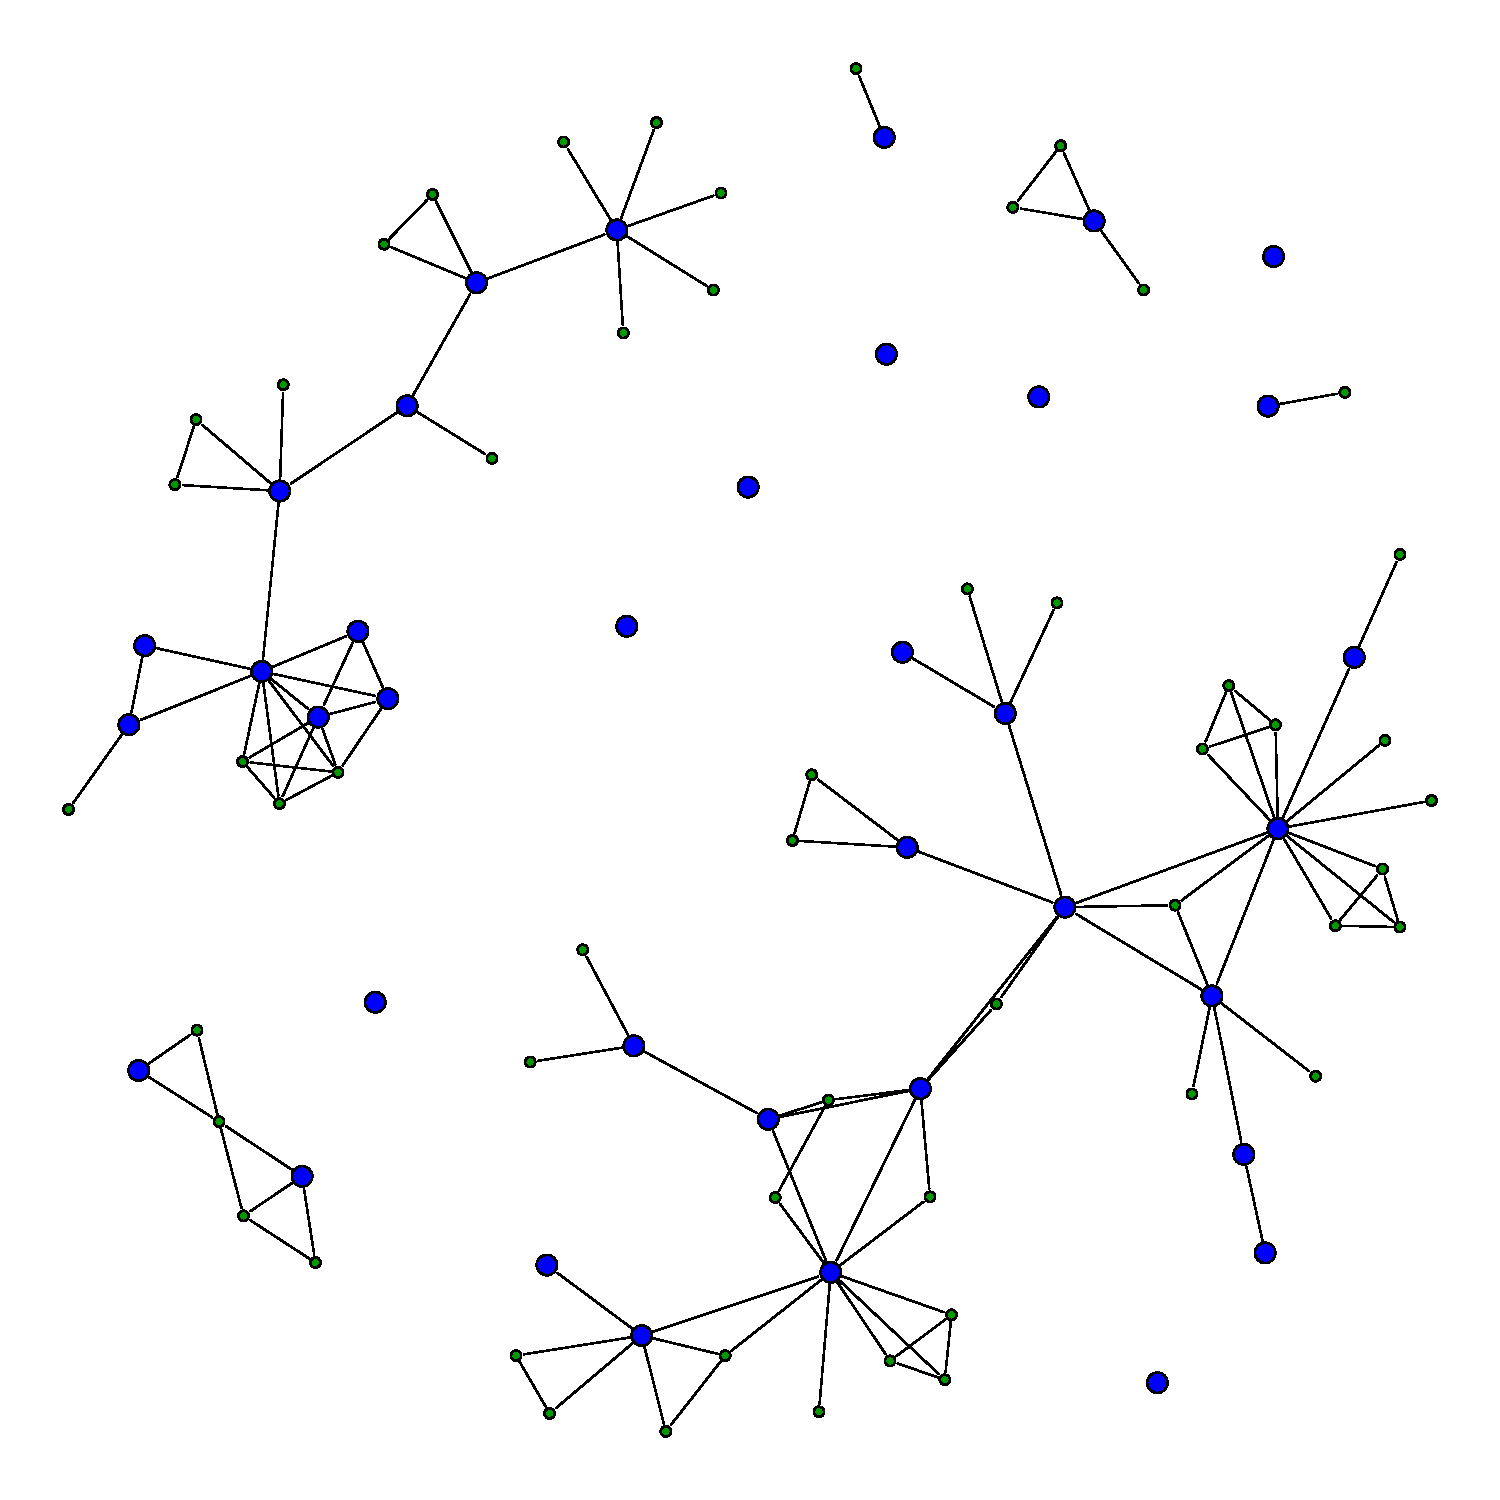
\includegraphics[width=5cm]{figuras/graph}
\caption{\label{fig:graph}Exemplo de uma figura.}
\end{figure}

\input sec-analise-ds-uio
\input sec-analise-hswitch
\input sec-analise-allpaths
